\section{Compressibility of Progressive Networks}

As described in the main text, one of the limitations of progressive networks is the growth in the size of the network with added tasks. In the basic approach we pursue in the main text, the number of hidden units and feature maps grows linearly with the number of columns, and the number of parameters grows quadratically.

Here, we sought to determine the degree to which this full capacity is actually used by the network. We leveraged the Average Fisher Sensitivity measure to study how increasing the number of columns in the Atari task set changes the need for additional resources. In Figure \ref{fig:app_compression}a, we measure the average fractional use of \textit{existing} feature maps in a given layer (here, layer 2). We do this for each network by concatenating the per-feature-map AFS values from all source columns in this layer, sorting the values to produce a spectrum, and then averaging across networks. We find that as the number of columns increases, the average spectrum becomes sparser: the network relies on a smaller proportion of features from the source columns. Similar results were found for all layers. 

Similarly, in Figure \ref{fig:app_compression}b, we measure the capacity required in the final added column as a function of the total number of columns. Again, we measure the spectrum of AFS values in an example layer, but here from only the final column. As the progressive network grows, the new column's features are both less important overall (indicated by the declining area under the graph), and have a sparser AFS spectrum. Combined, these results suggest that significant pruning of lateral connections is possible, and the quadratic growth of parameters might be contained.

\begin{figure}[h]
  \centering
    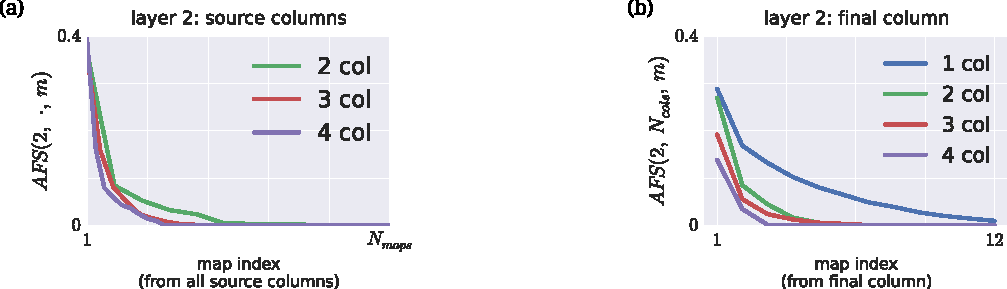
\includegraphics[width=.95\textwidth]{figures/appendix_compression.pdf}
    \caption{(a) Spectra of AFS values (for layer 2) across all feature maps from source columns, for the Atari dataset. The spectra show the range of AFS values, and are averaged across networks. While the 2 column / 3 column / 4 column nets all have different values of $N_{maps}$ (here, 12, 24, and 36 respectively), these have been dilated to fit the same axis to show the proportional use of these maps. (b) Spectra of AFS values (for layer 2) for the feature maps from only the final column. 
      }
    \label{fig:app_compression}
\end{figure}

